\documentclass[12pt]{article}
\usepackage{fontspec}

\setmainfont{Times New Roman} % Times New Roman, Arial, Calibri

\usepackage{setspace}
\setstretch{1.15}

\usepackage{graphicx}
%\usepackage[backend=biber, style=authoryear]{biblatex}
\usepackage[backend=biber, style=numeric]{biblatex}
\addbibresource{references.bib}

\usepackage{geometry}
\geometry{top=2.5cm, bottom=2.5cm, left=2.5cm, right=2.5cm}

\usepackage{pdfpages}

\usepackage{listings}
\usepackage{xcolor}
% Define colors
\definecolor{codegreen}{rgb}{0,0.6,0}
\definecolor{codegray}{rgb}{0.5,0.5,0.5}
\definecolor{codepurple}{rgb}{0.58,0,0.82}
\definecolor{backcolour}{rgb}{0.95,0.95,0.92}


\title{Identifying Dynamic Systems with Probabilistic Numerics}
\author{Harvey Walton}
\date{\today}

\begin{document}
    \pagenumbering{roman}

    \thispagestyle{empty}
    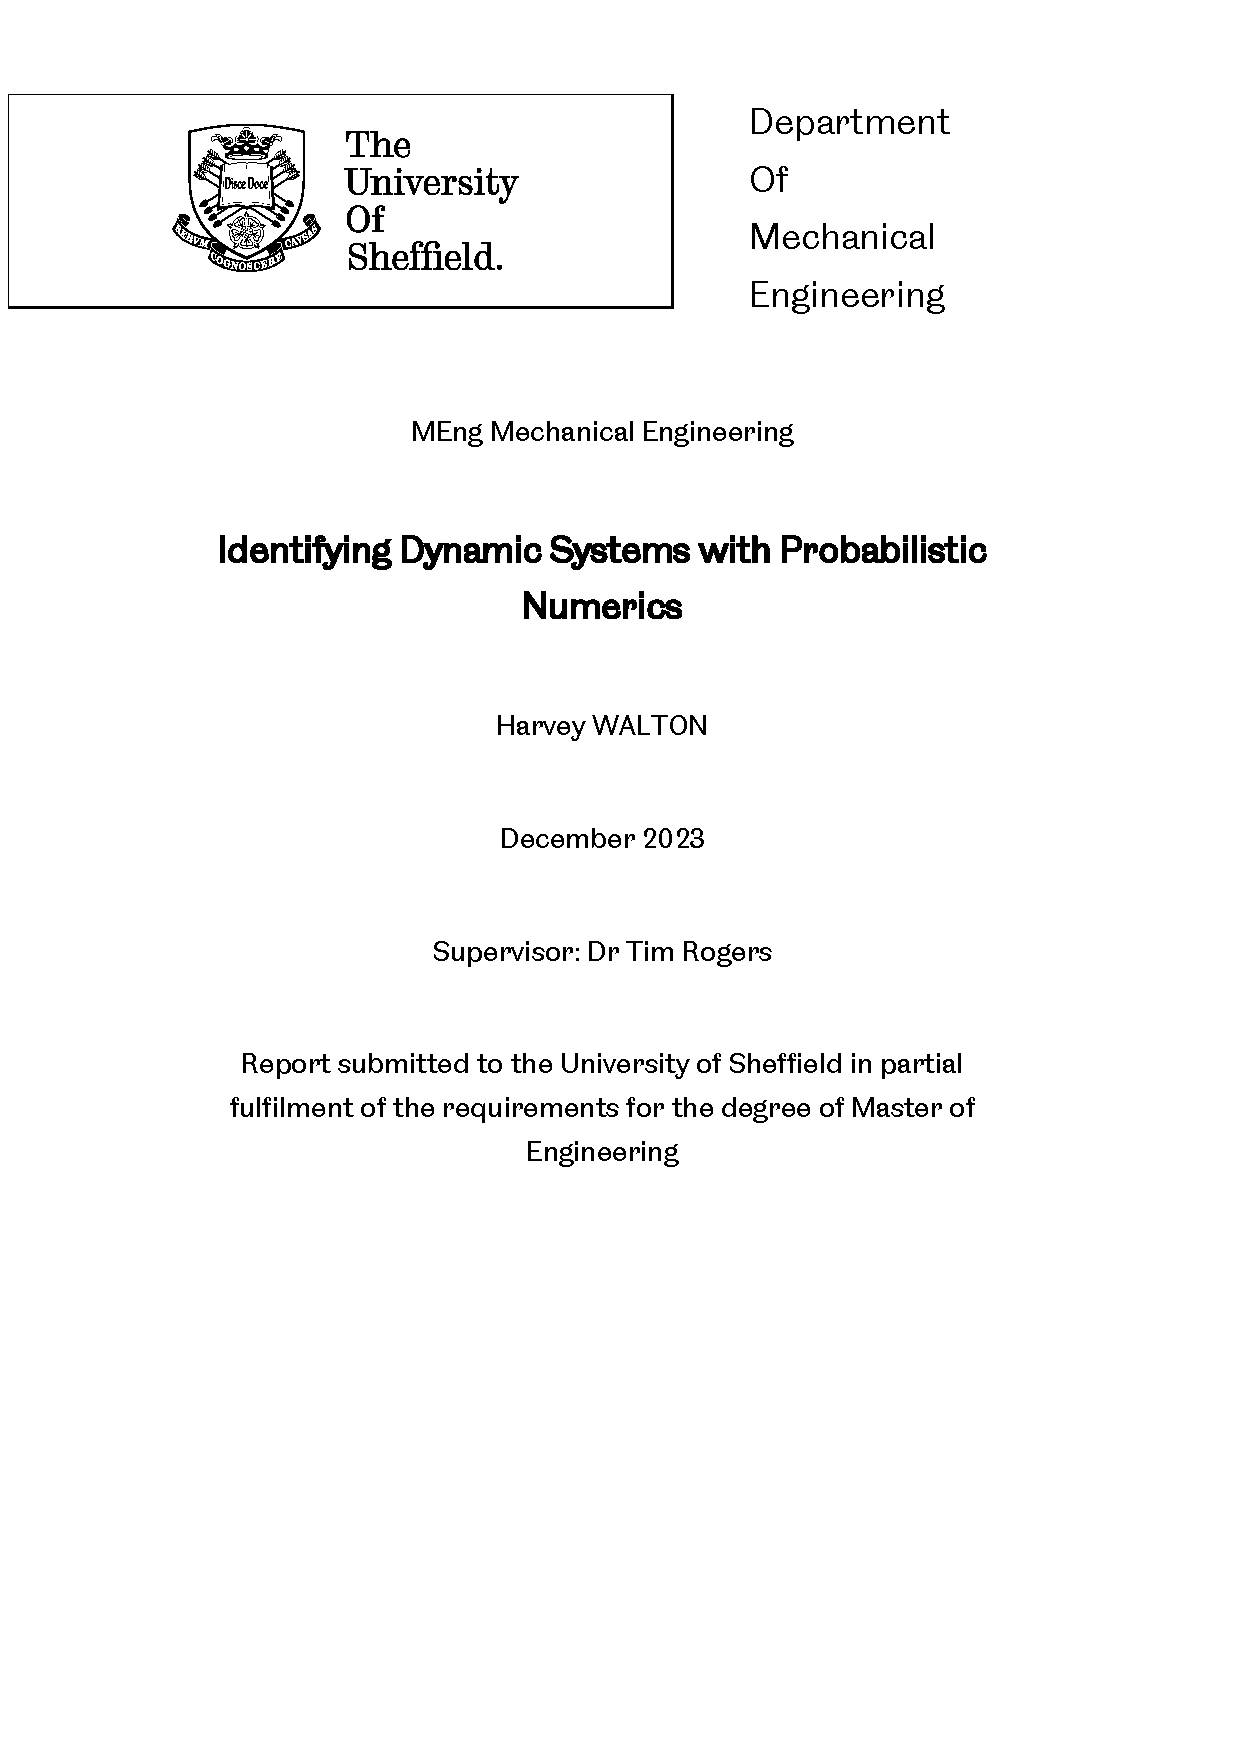
\includepdf[pages=1, frame, scale=1.09, pagecommand={}, offset=0 -35]{figures/titlepage.pdf}


    \tableofcontents
    \newpage

    \pagenumbering{arabic}

    \section{Background and Understanding of the Problem}


    Problems in engineering are usually described using a framework of continuous mathematical functions.
    This means that their output has no jumps or gaps in values, and they can be evaluated using input values that are on a sliding scale of a continuous input domain.
    For example, time in the real world is on a continuous sliding scale, which means that any interval in time can always be subdivided into a smaller interval.
    Continuous functions in turn can often be manipulated analytically using mathematics.
    For example, if the velocity of a particle is given as a continuous function of time, a continuous acceleration function can be derived from the velocity analytically through a mathematical process called differentiation.

    However, there are many situations where this analytical approach is unsuitable.
    The first reason for this is that the analytical approach may be too complex for anyone to have solved.
    A good example of this is the Gaussian (normal) distribution.
    This definite integral of this is often needed to be found in order to find the cumulative distribution function.
    This process can be visualised as finding the area underneath th


    However, to collect data for real world events, it must be sampled or else the amount of information needed to represent the event, as well as the amount of computing power to perform analysis on the event, would tend to infinity.
    Similarly, many problems in the real world are too complex to be solved analytically and so numerical methods are used to approximate the solution to these problems.
    However, what if there was a better approach?
    What if instead of resorting to numerical methods to solve the problem discretely, the original continous data could be reconstructed in "closed form".

        However, these methods are not perfect, and introduce error into the solutions.
        This error can be quantified, and is often done so using error bounds


    However, instead, what if the error was quantified using a probability distribution

    Instead, what if we use uncertainty define a pdf of result using (mean and standard deviation)
    in this case, it may be easier to quantify concepts like risk and improve automation of decision-making within engineering
    \subsection{}

    \section{Aims and Objectives}
    Your text goes here.

    \section{Work completed to date}
    Your text goes here. \cite{q-candela}
    \section{Plan for future work}
    Your text goes here.

    \appendix
    \section{The use of generative AI (ChatGPT)}
    ChatGPT was used to create some things:
    \subsection{inverse\_triangluar\_matrix\ function}
    Put prompt and output
    \subsection{Figures for the report}
    \subsubsection{Cumulative Distribution Function}
    Put prompt and output


    \printbibliography

\end{document}
